      
               
                \begin{ledgroupsized}[r]{120mm}
                \footnotesize 
                \pstart                
                \noindent\textbf{\"{U}berlieferung:}   
                \pend
                \end{ledgroupsized}
            
              
                            \begin{ledgroupsized}[r]{114mm}
                            \footnotesize 
                            \pstart \parindent -6mm
                            \makebox[6mm][l]{\textit{L}}Konzept: LH XXXV 12, 2 Bl. 62. 1 Bl. 15 x 17 cm. \nicefrac{1}{2} S. Auf der unteren H\"{a}lfte der Vorderseite unser St\"{u}ck. Dar\"{u}ber Bezeichnungen f\"{u}r mathematische Ausdr\"{u}cke, die in \cite{00115}\title{LSB} VII, 3 N. 38.16 gedruckt wurden. Die drei Zeilen des Textes etwa in der Mitte des Blattes. Links unterhalb des Textes drei Zeichnungen nebeneinander, davon die rechte gestrichen. Text auf Bl. 62~v\textsuperscript{o} in \cite{00115}\title{LSB} VII, 5 N. 9 gedruckt. Papier durch Erhaltungsma{\ss}nahmen stabilisiert.\\Cc 2 Nr. 543 \pend
                            \end{ledgroupsized}
                %\normalsize
                \vspace*{5mm}
                \begin{ledgroup}
                \footnotesize 
                \pstart
            \noindent\footnotesize{\textbf{Datierungsgr\"{u}nde}: Die Datierung des St\"{u}cks richtet sich nach derjenigen, die f\"{u}r \title[115]{LSB} VII, 5 N. 9 erfolgt ist sowie nach der dort gemachten Vermutung, dass Leibniz zurerst die mathematischen Aufzeichnung auf der R\"{u}ckseite von Bl. 62 verfasst habe. Das vorliegende St\"{u}ck k\"{o}nnte daher gleichfalls im Oktober 1674 oder wenig sp\"{a}ter entstanden sein.}
                \pend
                \end{ledgroup}
            
                \vspace*{8mm}
                \pstart 
                \normalsize
            \noindent[62~r\textsuperscript{o}]  Pendulorum longitudines duplicatam habent rationem temporum, quibus minimae vibrationes\protect\index{Sachverzeichnis}{vibratio} perficiuntur.\pend \pstart \vspace{2em} \begin{center}                    
                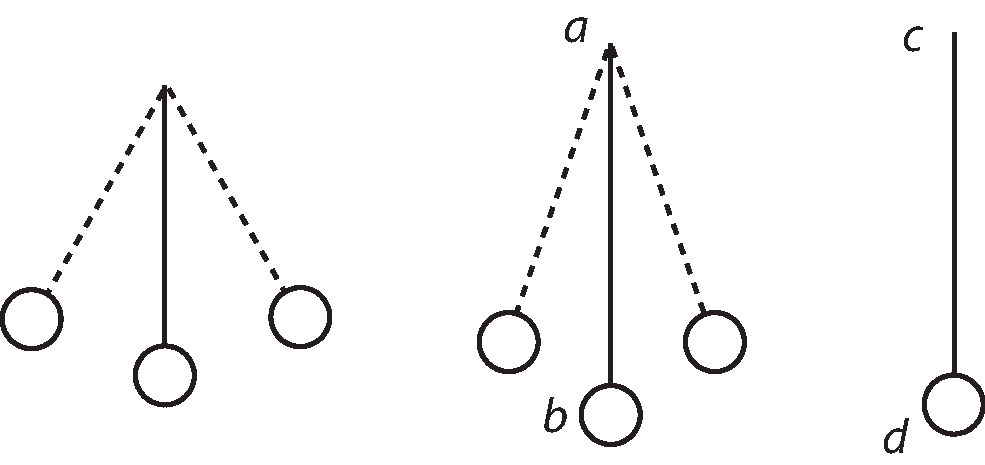
\includegraphics[width=0.6\textwidth]{images/62-123.pdf}
              
                      \textit{[Fig. 1]}\hspace*{4mm}  \textit{[Fig. 2]}\hspace*{4mm}  \textit{[Fig. 3, gestrichen]}
\vspace*{2mm}
                        \end{center}
                        %@ @ @ Dies ist eine Abstandszeile - fuer den Fall, dass mehrere figures hintereinander kommen, ohne dass dazwischen laengerer Text steht. Dies kann zu einer Fahlermeldung fuehren. @ @ @ \\
                   
                    \vspace{2em} \lbrack \textit{Rechnungsfragmente ohne Textbezug:}\rbrack \pend \pstart \vspace{1em} \begin{tabular}{c}
                                   1500\\
                                   1000\\
                                  \end{tabular}
                        %@ @ @ Dies ist eine Abstandszeile - fuer den Fall, dass mehrere figures hintereinander kommen, ohne dass dazwischen laengerer Text steht. Dies kann zu einer Fahlermeldung fuehren. @ @ @ \\
                    \begin{tabular}{cc}
                                  999 &333\\
                                 \end{tabular}
                        %@ @ @ Dies ist eine Abstandszeile - fuer den Fall, dass mehrere figures hintereinander kommen, ohne dass dazwischen laengerer Text steht. Dies kann zu einer Fahlermeldung fuehren. @ @ @ \\
                     \pend 
 


 


 


 


 

